%% LyX 2.3.1-1 created this file.  For more info, see http://www.lyx.org/.
%% Do not edit unless you really know what you are doing.
\documentclass{article}
\usepackage[latin9]{inputenc}
\usepackage{array}
\usepackage{multirow}
\usepackage{amsmath}
\usepackage{graphicx}
\usepackage{float}
\usepackage{subfigure}

\makeatletter

%%%%%%%%%%%%%%%%%%%%%%%%%%%%%% LyX specific LaTeX commands.
%% Because html converters don't know tabularnewline
\providecommand{\tabularnewline}{\\}
%% A simple dot to overcome graphicx limitations
\newcommand{\lyxdot}{.}


%%%%%%%%%%%%%%%%%%%%%%%%%%%%%% User specified LaTeX commands.



%%%%%%%%%%%%%%%%%%%%%%%%%%%%%% User specified LaTeX commands.
% Template for GlobalSIP-2018 paper; to be used with:
%          spconf.sty  - ICASSP/ICIP LaTeX style file, and
%          IEEEbib.bst - IEEE bibliography style file.
% --------------------------------------------------------------------------
\usepackage{spconf}


\def\x{{\mathbf x}}
\def\L{{\cal L}}

\makeatother 

\begin{document}
\title{     
  %SFC: Few-Shot Text Classification via Similarity Fused with Classification System
  Joint training of classification model and similarity model for low-resource
  text classification in chatbot
}
\name{Jingwen Huang}   
\address{     
  \{hanmei613\}@gmail.com   
}
\maketitle 

\begin{abstract}
  Building  conversational  chatbot  system  has  become  a  popular solution to customer  services  under various business scenarios. A
  conversational  chatbot needs to detect user's intent given a few words, which
  essentially  equals  to  short-text  classification  problem  in  the field of Natural  Language  Processing.  Moreover,  each  time  for  a  new service, the task-specific  chatbot  system  often needs to perform well in few-shot setups due  to lack of domain-specific data, which is quite a challenge for single-model system such as text classification model system or sentence-pair semantic similarity model system under such a low-resource condition. Therefore, in this paper, we propose
  SFC,  a 2-stage joint system with multi-task training technique for both text classification task and sentence-pair semantic similarity task to
  overcome  this challenge. Furthermore, we additionally propose an improved version of SFC to allow text classification model and sentence-pair model be combined into a joint model organized in hierarchical structure. We also
  conduct extensive experiments on 4 public and 1 private datasets in few-shot setup (i.e.,
  with only 5 to 20 training data per class). The experimental results show that
  our  system can steadily outperform several competitive single-model baselines by 2 percent
  in average accuracy.
\end{abstract}
%\keywords{}

\section{Introduction}
\label{sec:intro}
% latest version start
Task-specific conversational chatbot\cite{wen2016network} are designed to share the working pressure of human customer service agents who are responsible for solving customers' questions or queries about certain products or services. Regardless of whether the conversation is single-turn or multi-turn, the essential technical solution behind the chatbot is intent classification model which can identify the correct intent behind user's input text and find the corresponding answer. 

Although task-specific conversational chatbot already has a wide application in various business and industries, it's still a quite challenging task due to its natural properties of low-resource. First, customers' utterance within a conversation is usually quite short and completed in a few words. Short text\cite{song2014short} are generally more ambiguous in comparison with long texts such as paragraphs or documents since they don't contain enough contextual information, which poses a great challenge\cite{chen2019deep} for classification task\cite{phan2008learning,yan2009dynamic,hua2015short}. Second, at the initial stage of building a chatbot for specific task or service, it's often extremely hard to collect sufficient data samples for each class. The reason is that it's usually too expensive and time consuming to extract different ways of natural language expression for each intent class from history conversation log or even manually compose the corpus from nothing. Therefore, the key to building a task-specific chatbot with high performance becomes solving the challenge of short-text classification\cite{sriram2010short} problem under few-shot setting\cite{yu2018diverse}.

\begin{figure}[htbp]
\centering 
\subfigure[classification model]{
\label{Fig.1.sub.1}
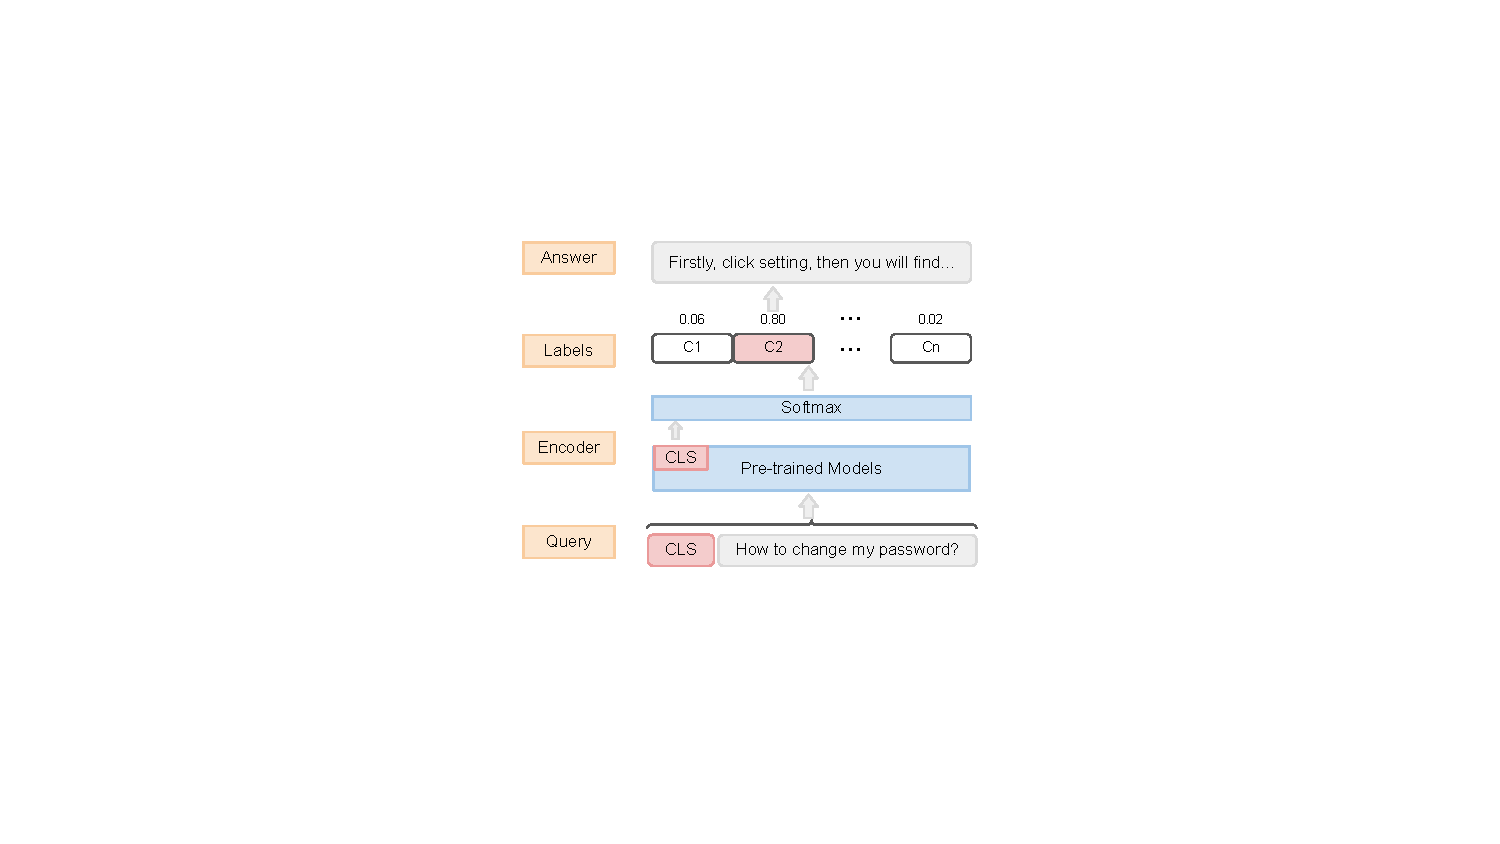
\includegraphics[scale=0.7]{picture1.pdf}}
\subfigure[similarity model]{
\label{Fig.1.sub.2}
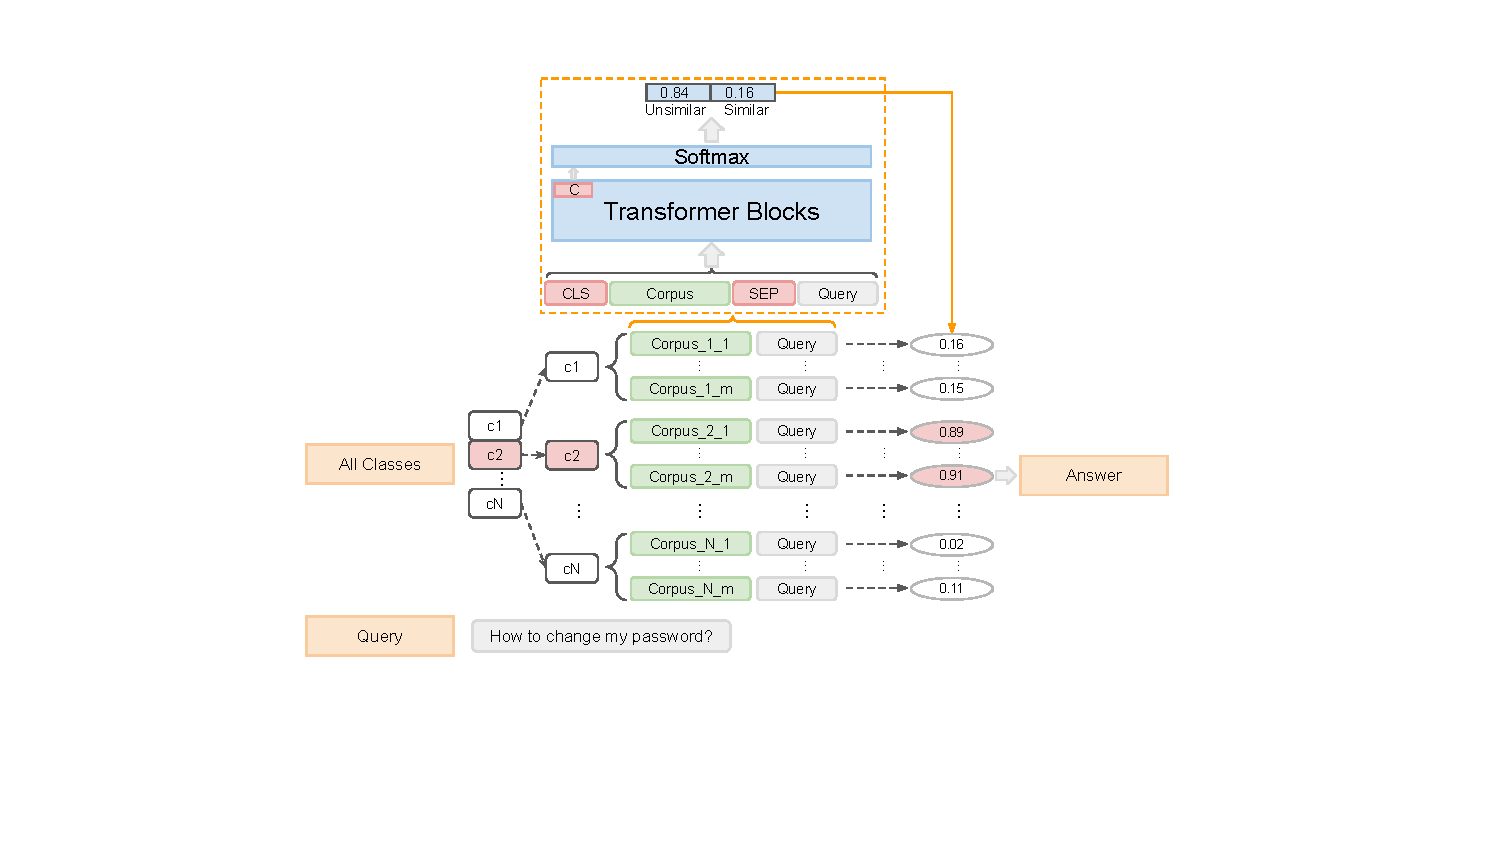
\includegraphics[scale=0.55]{picture2.pdf}}
\caption{Two popular structures of building task-specific conversational chatbot}
\label{Fig.1.main}
\end{figure}

One of the most popular approach among existing work was text classification model based on neural network. Since the length of the text is quite short, many previous work\cite{wen2016network} choose neural network such as convolutional neural networks (CNNs)\cite{kim2014convolutional,zhang2015character,conneau2016very}
or long short term memory networks
(LSTMs)\cite{mousa2017contextual,liu2016recurrent} to accomplish the task of extracting semantic feature from limited amount of words. A common model structure is adding a softmax classifier to the top of the neural network. Afterwards, pre-trained language models on large corpus like BERT\cite{devlin2018bert} and
RoBERTa\cite{liu2019roberta} has  been proven more powerful in solving many NLP
tasks      including      short-text      classification\cite{madabushi2020cost}.   Especially   for  few-shot  scenarios\cite{yu2018diverse}, pre-trained  model  based on transformers\cite{vaswani2017attention}, shown in Fig. \ref{Fig.1.sub.1}, tends  to  do more help to reducing the negative effects brought by scarcity of training data. 

Another popular approach among previous work was based on sentence-pair model. The motivation of this approach was started from the idea of Information Retrival (IR) based chatbot\cite{jafarpour2010filter, leuski2011npceditor}. Having a Q-A (Question-Answer) pairs dataset and user query Q, the IR based conversational system will look up in the Q-A dataset for the pair (Q', A') that best matches query Q through semantic analysis and returns A' as the answer to Q\cite{mnasri2019recent}. In this way, sentence-pair model pre-trained on large corpus of semantic similarity identification task can be applied for being used as a tool to identify the class with highest semantic similarity to customer's query. A common model structure of pre-trained\cite{devlin2018bert} sentence-pair model is based on multiple cross-attention mechanism\cite{barkan2020scalable}, shown in Fig. \ref{Fig.1.sub.2}. Due to the fact that many experiment results have shown that RoBERTa\cite{liu2019roberta} is an improved  version  of  BERT, and has achieved amazing results on both text classification and sentence-pairs semantic similarity tasks, we choose RoBERTa as an important baseline approach in this paper.

Despite the success of these 2 approaches, they still have some limitations in task-specific chatbot scenario. As for the text classification model approach, it's quite hard to use data augmentation method to solve the data insufficiency challenge since the it's usually unfeasible to get large amount of domain-specific data when facing a new task. With respect to the sentence-pair model approach, though we can obtain large amount of data in semantically duplicate sentence pair identification domain for transfer learning\cite{sun2019fine}, it's still quite hard to perform well on task-specific dataset because the training objective of sentence-pair model is semantic similarity, which is slightly different from the target of classification task. That is to say, there always exists some intent classes which cannot be distinguished by each other merely depending on semantic similarity. For example, we have 2 user query saying, A: What should I do if I want to change my password? B: What is the modification rule if I want to change my password? In this case, sentence A is semantically similar to B, since they both express the 
desire for changing password. However, it's still reasonable to classify them into 2 intent classes, since A is asking for the method for changing password, while B is asking for the rule to follow when creating a new password.

\begin{figure}[htbp]
\begin{centering}
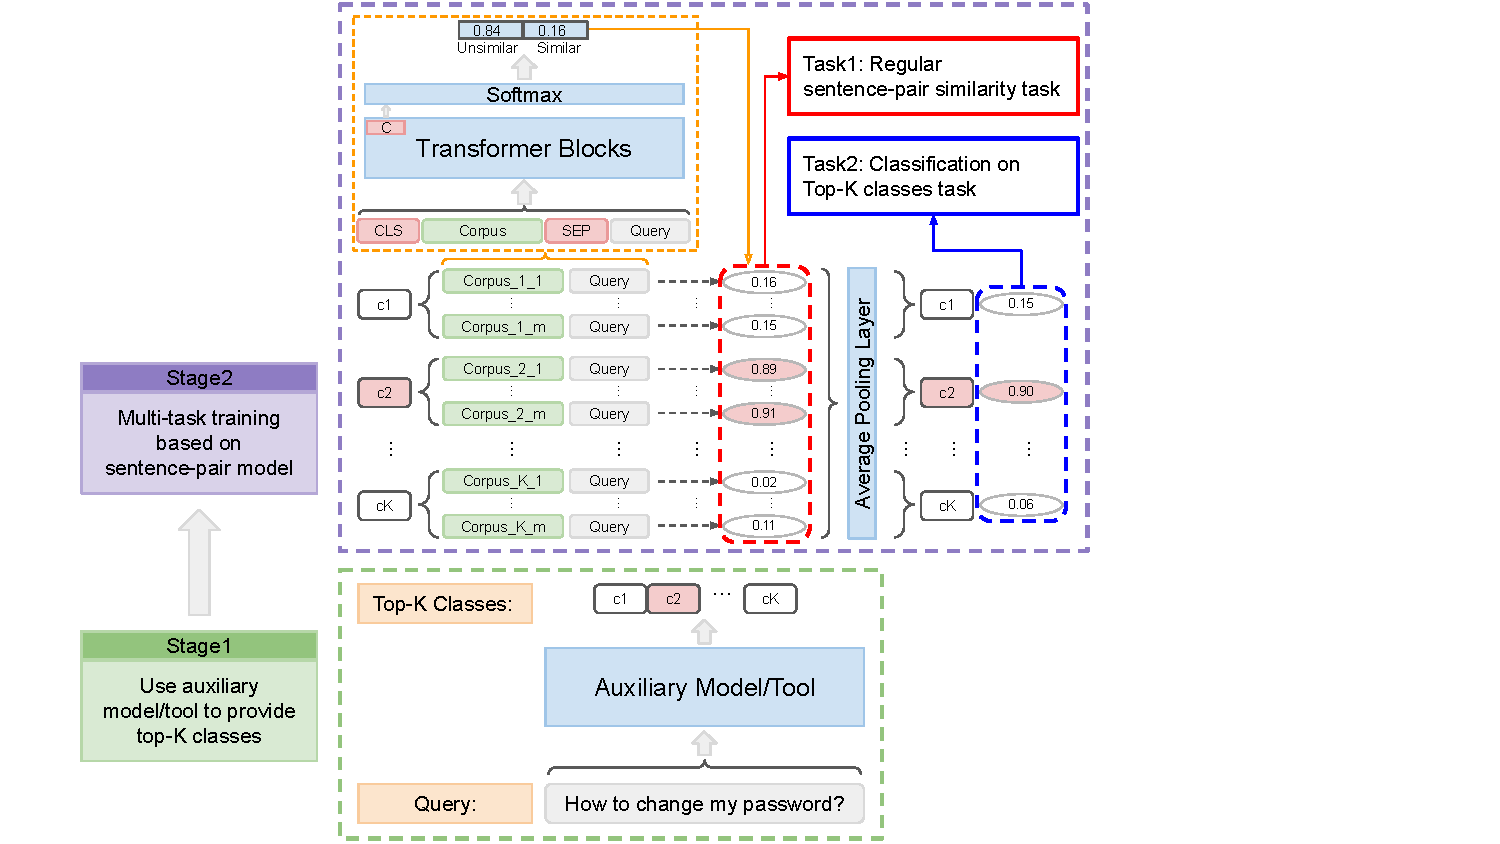
\includegraphics[scale=0.48]{picture3}
\par\end{centering}
\caption{\textbf{Network Structure of 2-stage SFC:} a joint system of multi-task for both text classification task and sentence-pair semantic similarity task.}
\label{fig:ver.1.3}
\end{figure}

The above limitation motivates us to propose a joint system of both text classification task and sentence-pair semantic similarity task, named SFC here, shown in Fig. \ref{fig:ver.1.3}. Our goal is to utilize the advantage of the feasibility of transfer learning based on semantic similarity, while in the mean time, add the classification task's target into the training process of sentence-pair model for multi-task learning\cite{caruana1993multitask,collobert2008unified}. To obtain such a joint system, we first start with preparation work, which is pre-training a sentence-pair model on external corpus for sentence pair duplication identification, and then find an auxiliary model or tool which can help us sample out top-K most related intent classes. This auxiliary model or tool can either be searching engine such as elasticsearch\cite{divya2013elasticsearch} or a text classification model trained on task-specific chatbot data. Afterwards, we further fine-tune the sentence-pair model with 2 training tasks: 1) the regular sentence pair similarity tasks. Here we use the text classification model as an auxiliary model in this paper to sample sentence pairs for training based on negative sampling strategy\cite{bamler2020extreme}. The reason is that a task-specific chatbot often has hundreds of intent classes, which forms too many sentence pairs for training since any two sentences from two different classes can form a sentence-pair of negative sample. Besides, according to Bamler\cite{bamler2020extreme}, training on negative samples from most confusing wrong label can help model converge faster and obtain better performance. 2) the classification task on top-K (here K is a hyperparameter) candidate classes provided by our auxiliary model or tool. Here we use the average pooling of the representation given by sentence-pair model for sentence pairs formed by the user input query and the corpus sentences in each class as the feature. We stack the task-specific layers on the top of the shared-parameter sentence-pair model structure, which is a classic parameter sharing mechanism\cite{collobert2008unified, subramanian2018learning,liu2019multi} for multi-task\cite{sun2019fine}. In this way, specific knowledge contained in these 2 tasks can be fully explored and deeply interact with each other to obtain better overall performance.

However, since the auxiliary tool in joint system mentioned above works in a separate stage from sentence-pair model, we find the the quality of sampled candidate classes might limit the overall performance of SFC, since the candidate classes for each user query is always fixed during the multi-task training process. This observation motivates us to further improve SFC into a joint model of sentence-pair model and text classification model in a hierarchical architecture by putting different tasks at different network layers\cite{sogaard2016deep, hashimoto2016joint} and then training them together, shown in Fig \ref{fig:framework}. Here, the text classification model involved in joint training process replace the role of auxiliary tools. In this way, the sentence pairs selected from top-K classes becomes dynamic, which means the text classification model will also be further optimized to provide better top-K classes pooling result.

We summarize our contributions as follow:

1) We propose a novel joint system named SFC with multi-task training technique designed for task-specific conversational chatbot with low-resource, in which we make full utilization of the advantages brought by both the text classification task and sentence-pair semantic similarity task.

2) To further improve the system performance of SFC, we also propose an innovative joint model structure, in which the text classification model and sentence-pair model are fused into one single model for joint training.

3) Experiment results on 4 public and 1 private short-text classification datasets with respect to intent recognition tasks under conversational chatbot scenario all demonstrated that our proposed SFC joint system with multi-task, as well as the improved version of SFC, can both achieve remarkable improvement comparing to some powerful single-task and single-model baselines, especially under few-shot settings. 

\begin{figure*}[t]
\begin{centering}
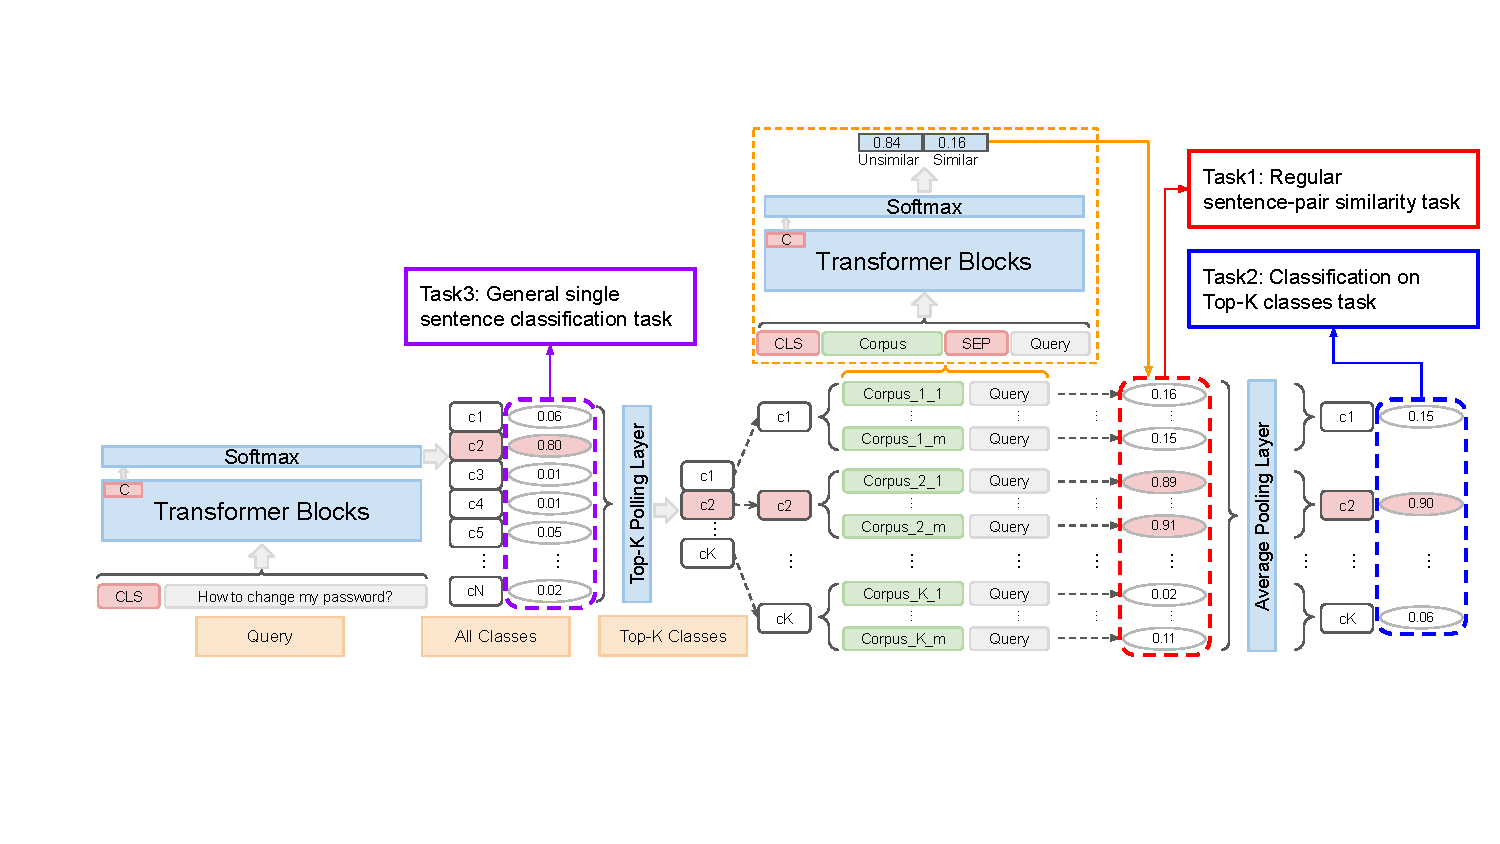
\includegraphics[scale=0.72]{picture4} 
\par\end{centering}
\caption{\textbf{Network Structure of hierarchical SFC:} a joint model of sentence-pair model and text classification model organized in hierarchical structure by completing different tasks at different network layers.}
\label{fig:framework}
\end{figure*}

% latest version end

%\section{Attention based neural network}

%\section{Conclusion}


\bibliographystyle{IEEEbib}
\bibliography{refs}

\end{document}
